\documentclass{../lab_class}

\usepackage{fancyhdr}
\pagestyle{fancy}
\rhead{П.\,Ю. Смирнов, 687 гр.}
\lhead{Лабораторная работа № 3.4.1, МФТИ, осень 2017}

\newcommand{\magm}{\mathfrak{m}}

\begin{document}

{\Large 3.4.1 -- Диа- и парамагнетики.}

\paragraph{Цель работы.}
Измерение магнитной восприимчивости диа- и парамагнетного образцов.
В работе используются: электромагнит, аналитические весы, милливеберметр, амперметр постоянного тока, реостаты, образцы.

\paragraph{Теоретическая часть.}

\begin{wrapfigure}[12]{r}{6cm}
\centering
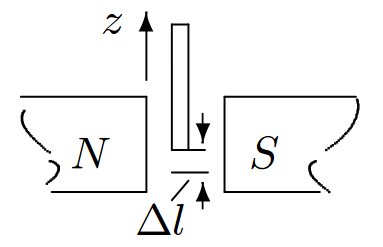
\includegraphics[width=5cm]{electromagnet.png}
\caption{Образец в электромагните}
\end{wrapfigure}

Рассмотрим два крупных класса веществ относительно их поведения в магнитном поле. Суммарный магнитный момент электронов в атомах \emph{диамагнетиков} в отсутствие внешнего магнитного поля равен нулю; при внесении вещества в магнитное поле возникают индуцированные атомные токи, создающие магнитные момент, направленный противоположно внешнему полю (проявление принципа Ле-Шателье). Атомы \emph{парамагнетика} же обладают собственными магнитными моментами, которые под действием внешних полей ориентируются по полю и тем самым создают результирующее поле, превышающее внешнее.

\begin{wrapfigure}[12]{l}{6cm}
\centering
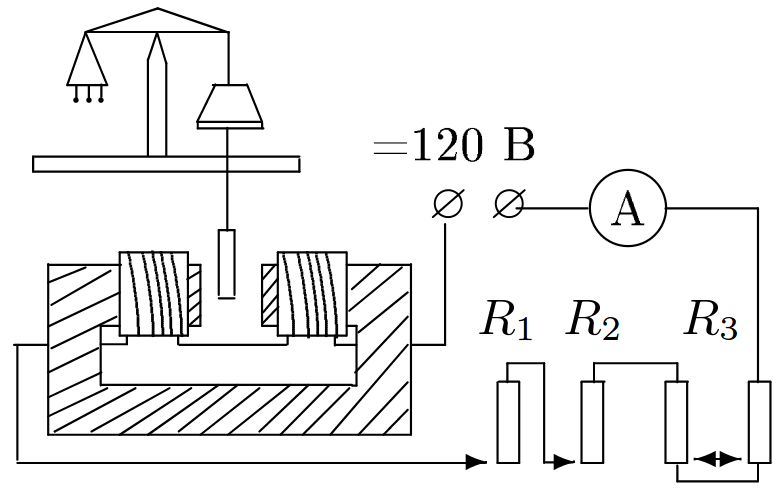
\includegraphics[width=5cm]{lab_scheme.png}
\caption{Схема экспериментальной установки}
\end{wrapfigure}

Для широкого класса веществ намагниченность (суммарный магнитный момент единицы объема вещества) и напряженность магнитного поля связаны линейно:
\begin{equation}
	\vb{M} = \chi \vb{H},
\end{equation}
где $\chi$ -- магнитная восприимчивость (скаляр, а не тензор!). Для парамагнетиков $\chi > 0$, диамагнетиков -- $\chi < 0$.

В данной работе предлагается измерить магнитную восприимчивость различных материалов, используя \emph{метод Гюи}. Тонкий длинный образец вещества вносится в узкий зазор электромагнита, измеряется сила, действующая на него со стороны поля. Найдем связь магнитной восприимчивости и силы. При смещении образца на $\Delta l$ магнитная сила есть
\begin{equation}
	F = \frac{\Delta W}{\Delta l},
\end{equation}
где $\Delta W$ -- изменение энергии поля. Магнитная энергия есть
\begin{equation}
	W = \frac{1}{2} \int H B \dd{V} = \frac{1}{2\mu_0} \int \frac{B^2}{\mu} \dd{V},
\end{equation}
где интеграл берётся по всему пространству. При смещении образца внутрь зазора поле около верхнего конца поля остаётся практически неизменным. Принимая поле внутри стержня равным измеренному наму полю в зазоре, получим
\begin{equation}
	\Delta W = \frac{1}{2\mu_0} \frac{B^2}{\mu} s \Delta l - \frac{1}{2\mu_0} B^2 s \Delta l = -\frac{\chi}{2\mu_0\mu} B^2 s \Delta l;
\end{equation}
отсюда следует, что на образец действует сила
\begin{equation}\label{eq:main}
	F = -\frac{\chi}{2\mu_0\mu} B^2 s.
\end{equation}

В нашей работе сила определяется с помощью аналитических весов. Мы исследуем три образца -- медь, алюминий, графит.

\paragraph{Результаты эксперимента.}

Построим градуировочную кривую для электромагнита. Калибровку мы проводим милливеберметром, измеряющим магнитный поток $\Phi = B S n$, где $S n = 72 \ \cm^2$. Отсюда получаем $B = f(I)$:

\begin{figure}[H]
\centering
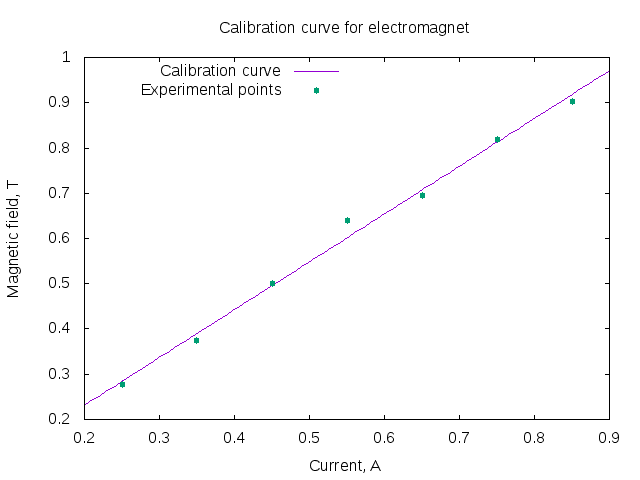
\includegraphics[width = 0.87 \textwidth]{calibration_curve.png}
\caption{Калибровочная кривая электромагнита, $k = 1.05 \pm 0.04 \ \T / \A$.}
\end{figure}

\bigskip

\begin{table}[H]
\centering
\begin{tabular}{|c|c|c|c|c|c|}
\hline
\multicolumn{2}{|c|}{Медь} &\multicolumn{2}{c|}{Алюминий} &\multicolumn{2}{|c|}{Графит}	\\ \hline
$I, \A$ &$m, \sm \g$ &$I, \A$ &$m, \sm \g$ &$I, \A$ &$m, \sm \g$	\\ \hline
1.17 &-35 &1.17 &76 &1.17 &-187	\\ \hline
0.94 &-27 &0.98 &62 &0.92 &-141	\\ \hline
0.77 &-20 &0.76 &42 &0.74 &-98		\\ \hline
0.62 &-14 &0.59 &26 &0.54 &-54		\\ \hline
0.49 &-9  &0.44 &15 &0.40 &-32		\\ \hline
0.31 &-4  &0.29 &6  &0.21 &-10		\\ \hline
\end{tabular}
\caption{Экспериментальные данные.}
\end{table}

Отрицательная масса здесь, конечно, свидетельствует не о существовании антимассы, а о том, что сила направлена противоположно вектору $\vb{g}$.

\begin{figure}[H]
\centering
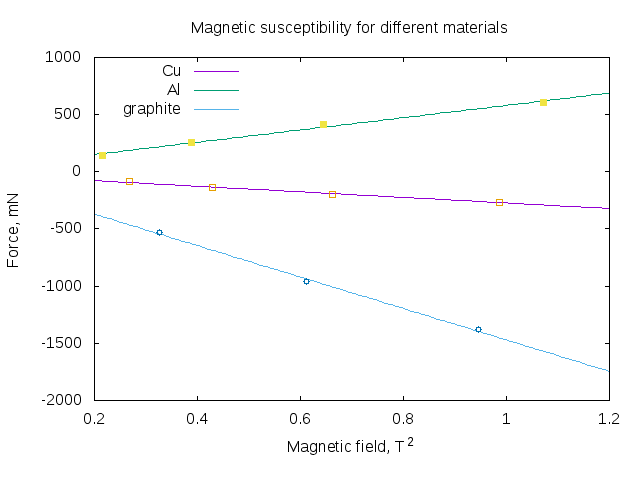
\includegraphics[width = 0.87 \textwidth]{graph.png}
\caption{Магнитная восприимчивость различных веществ.}
\end{figure}

По полученному наклону прямой мы можем, используя формулу \ref{eq:main}, найти магнитную восприимчивость материала. Стержни представляют собой цилиндры диаметрами $d = 10 \ \mm$ для меди, $d = 10 \ \mm$ для алюминия и $d = 6.7 \ \mm$ для графита соответственно. Отсюда получаем:
\begin{gather*}
	\chi_{\text{Cu}} = (-7.8 \pm 0.5) \times 10^{-9} \ \m^3/\kg \\
	\chi_{\text{Al}} = (17 \pm 0.6) \times 10^{-9} \ \m^3/\kg \\
	\chi_{\text{graphite}} = (-0.98 \pm 0.5) \times 10^{-7} \ \m^3/\kg.
\end{gather*}
Между тем табличные данные есть $\chi_{\text{Cu}} = -1.13 \times 10^{-9} \ \m^3/\kg$, $\chi_{\text{Al}} = 7.54 \times 10^{-9} \ \m^3/\kg$, $\chi_{\text{graphite}} = -3.6 \times 10^{-7} \ \m^3/\kg$.

\paragraph{Вывод.}
Метод Гюи доказал свою применимость на практике и позволил измерить магнитную восприимчивость нескольких материалов в пределах известной погрешности. Кроме того, мы установили, что медь и графит -- диамагнетики, а алюминий -- парамагнетик.

\end{document}